This section deals with the new SmartRobotinoMPSDocking component. The new docking algorithm is discussed in this chapter, including the advantages and disadvantages of the new approach.

\subsubsection{Overview}

The new docking approach is much more lightweight than the old one from 2017.

\begin{figure}[h]
\centering
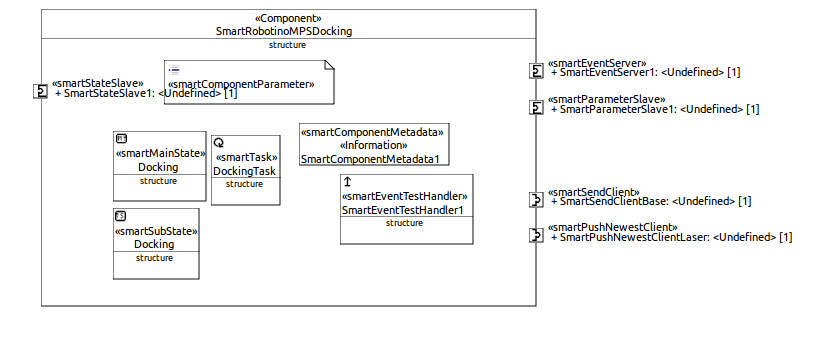
\includegraphics[scale=0.4]{pic/dockingComponent.png}
\caption{Model of the new Docking Component }
\label{fig:i_overview}
\end{figure}

The component consists mainly of one task (e.g. DockingTask), which just performs the docking to the corners of a MPS station, provided by the detection component.

\subsubsection{Old Version 2017}

The docking procedure of the former team was part of the SmartMPSDockingRoboCup component, which combined the detection task with the docking task.
The docking algorithm is implemented in a very incomprehensible way and also provides random docking results. Therefore the team of 2018 implemented a complete new docking component, which is lightweight, easy to understand and simple to optimize.

\subsubsection{New Version 2018}

For the new docking approach the two corners of the target MPS station is enough information. The docking task performs the following procedure:

\begin{enumerate}
\item Turn towards the target MPS station
\item Calculate the angle between robot and MPS station
\item Turn left or right until angle of robot to station is around 90 degree
\item Drive towards the middle of the MPS station, while angle to station is around 90 degree
\end{enumerate}

The calculation of the angle between robot and the target MPS station is described in the next paragraph. The other points of the procedure are descriptive to the enumeration above implemented.

\paragraph{Calculation of the angle between robot and MPS}

\begin{equation}
\cos(\phi) = \frac{ \vert \overrightarrow{roboDirectionVector} \circ \overrightarrow{stationVector} \vert} { \vert \overrightarrow{roboDirectionVector}  \vert  \cdot \vert \overrightarrow{stationVector}  \vert}
\end{equation}

\begin{equation}
\phi = \cos ^{ - 1} \left( \frac{ \vert \overrightarrow{roboDirectionVector} \circ \overrightarrow{stationVector} \vert} { \vert \overrightarrow{roboDirectionVector}  \vert  \cdot \vert \overrightarrow{stationVector}  \vert} \right)
\end{equation}

test



